\documentclass[11pt]{beamer}

\usetheme[]{Marburg}
\definecolor{backgr}{rgb}{0,0.4,0.8}
\usecolortheme[] {seahorse}

\usepackage[utf8]{inputenc} 
\usepackage[english]{babel}   %for protocosl in Englisch    %für Protokolle in Englisch 
\usepackage{amsmath}
\usepackage{amssymb}

%for listings  %zum Einbinden von Programmcode
\usepackage{listings}
\renewcommand{\lstlistingname}{Listing}
\usepackage{xcolor} 
\definecolor{hellgelb}{rgb}{1,1,0.9}
\definecolor{colKeys}{rgb}{0,0,1}
\definecolor{colIdentifier}{rgb}{0,0,0}
\definecolor{colComments}{rgb}{1,0,0}
\definecolor{colString}{rgb}{0,0.5,0}
\definecolor{dkgreen}{rgb}{0,0.6,0}
\definecolor{gray}{rgb}{0.5,0.5,0.5}
\definecolor{mauve}{rgb}{0.58,0,0.82}

\let\oldsqrt\sqrt
\def\sqrt{\mathpalette\DHLhksqrt}
\def\DHLhksqrt#1#2{%
	\setbox0=\hbox{$#1\oldsqrt{#2\,}$}\dimen0=\ht0
	\advance\dimen0-0.2\ht0
	\setbox2=\hbox{\vrule height\ht0 depth -\dimen0}%
	{\box0\lower0.4pt\box2}}

\lstset{ %
  language=Matlab,                    % the language of the code
  basicstyle=\footnotesize,           % the size of the fonts that are used for the code
  numbers=left,                       % where to put the line-numbers
  numberstyle=\color{gray},           % the style that is used for the line-numbers
  stepnumber=1,                       % the step between two line-numbers. If it's 1, each line 
                                      % will be numbered
  numbersep=5pt,                  % how far the line-numbers are from the code
  backgroundcolor=\color{hellgelb},      % choose the background color. You must add \usepackage{color}
  showspaces=false,               % show spaces adding particular underscores
  showstringspaces=false,         % underline spaces within strings
  showtabs=false,                 % show tabs within strings adding particular underscores
  frame=single,                   % adds a frame around the code
  rulecolor=\color{black},        % if not set, the frame-color may be changed on line-breaks within not-black text (e.g. comments (green here))
  tabsize=1,                      % sets default tabsize to 2 spaces
 captionpos=b,                    % sets the caption-position to bottom
  breaklines=true,                % sets automatic line breaking
  breakatwhitespace=false,        % sets if automatic breaks should only happen at whitespace
  caption=\lstname,               % show the filename of files included with \lstinputlisting;
                                  % also try caption instead of title
  keywordstyle=\color{blue},          % keyword style
  commentstyle=\color{dkgreen},       % comment style
  stringstyle=\color{mauve},          % string literal style
  escapeinside={\%*}{*)},             % if you want to add LaTeX within your code
  morekeywords={break,case,catch,continue,else,elseif,end,for,function,
   global,if,otherwise,persistent,return,switch,try,while,ones,zeros,tf,ss,jacobian,double,subs,freqz,fvtool,bode,syms},              % if you want to add more keywords to the set
  deletekeywords={...}              % if you want to delete keywords from the given language
}

\usepackage[e]{esvect}





\usepackage[update,prepend]{epstopdf}

\usepackage{hyperref}

%now the document
\begin{document}

\title{Flyball Governor}   
\author{Eda Sevim \\ Tobias Karg} 
%\titlegraphic{\input{pics/fh_image.tex}}
\institute{Dynamic Models \& Simulation}
\date{\today}
\begin{frame}
	\titlepage
\end{frame}

%\hypersetup{linkbordercolor=white}
\section{System Description}
\begin{frame}{System Description}
	\subsection{System Overview}
	\framesubtitle{System Overview}
	\begin{figure}[H]
		\centering
		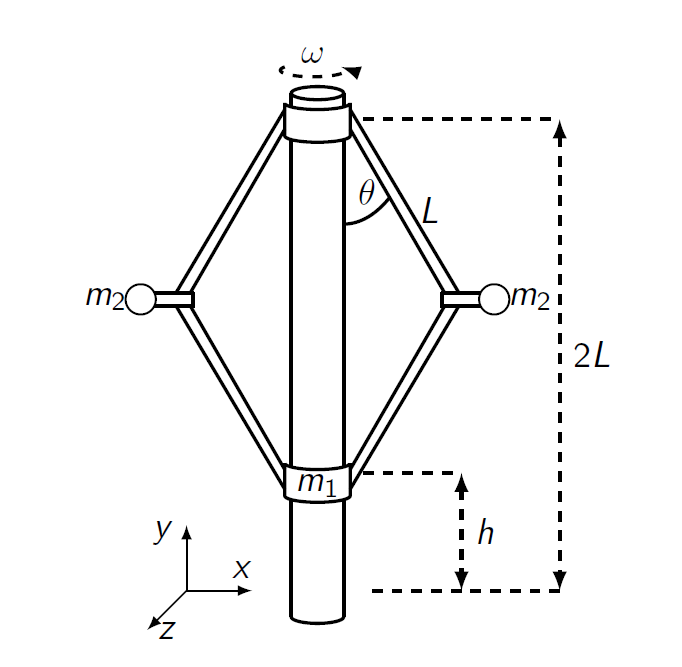
\includegraphics[width=0.80\textwidth]{pics/overview.png}
	\end{figure}
\end{frame}

\subsection{Position Vectors}
\begin{frame}{System Description}
	\framesubtitle{Position Vectors}
	\begin{equation*}
	\vv{r}_{m2,1} = \left(\begin{array}{c}
	L\sin(\theta)\cos(\beta)\\ L(2-\cos(\theta)) \\ -L\sin(\theta)\sin(\beta)
	\end{array}\right)
	\end{equation*}
	\begin{equation*}
	\vv{r}_{m2,2} = \left(\begin{array}{c}
	-L\sin(\theta)\cos(\beta)\\ L(2-\cos(\theta)) \\ L\sin(\theta)\sin(\beta)
	\end{array}\right)
	\end{equation*}
	\begin{equation*}
	\vv{r}_{m1} = \left(\begin{array}{c}
	0\\ 2L(1-\cos(\theta)) \\ 0
	\end{array}\right)
	\end{equation*}
	\centering mit $\beta = \int \omega dt$
\end{frame}
\section{System Dynamics}
\subsection{Energies}
\begin{frame}{System Dynamics}
	\framesubtitle{Kinetic Energy $T$ and Potential Energy $V$}
	\begin{equation*}
		T = \frac{m_1\|\dot{\vv{r}}_{m1}\|^2}{2} + \frac{m_2\|\dot{\vv{r}}_{m2,1}\|^2}{2} + \frac{m_2\|\dot{\vv{r}}_{m2,2}\|^2}{2}
	\end{equation*}
	\begin{equation*}
		T = 2m_1L^2\sin^2(\theta)\dot{\theta}^2 + m_2L^2\dot{\theta}^2 + m_2L^2\sin^2(\theta)\omega^2
	\end{equation*}\\

	\begin{equation*}
		V = m_1gh_1 + m_2gh_{2,1} + m_2gh_{2,2}
	\end{equation*}
	\begin{equation*}
		V = 2m_1gL(1-\cos(\theta)) + 2m_2gL(2-\cos(\theta))
	\end{equation*}
\end{frame}

\subsection{Result}
\begin{frame}{System Dynamics}
	\framesubtitle{Result}
	\begin{equation*}
			\ddot{\theta} = \frac{\sin(2\theta)(\frac{m_2}{2}\omega^2-m_1\dot{\theta}^2) - \frac{g}{L}\sin(\theta)(m_1 + m_2)}{m_2 + 2 m_1 \sin(\theta)^2}
	\end{equation*}
\end{frame}
%\section{Simulation}
\subsection{Simulation}
\begin{frame}{System Dynamics}
	\framesubtitle{Simulation}
	\begin{figure}[H]
		\centering
		$m_1 = 1\,\left[\mathrm{kg}\right]$, $m_2 = 2\,\left[\mathrm{kg}\right]$, $L = 0.4\,\left[\mathrm{m}\right]$, $\omega = 3\pi\,\left[\mathrm{\frac{rad}{s}}\right]$, $x_0 = \left(\begin{array}{c c}
		1 & 0
		\end{array}\right)^T$\\
		\begin{figure}[H]
			\centering
			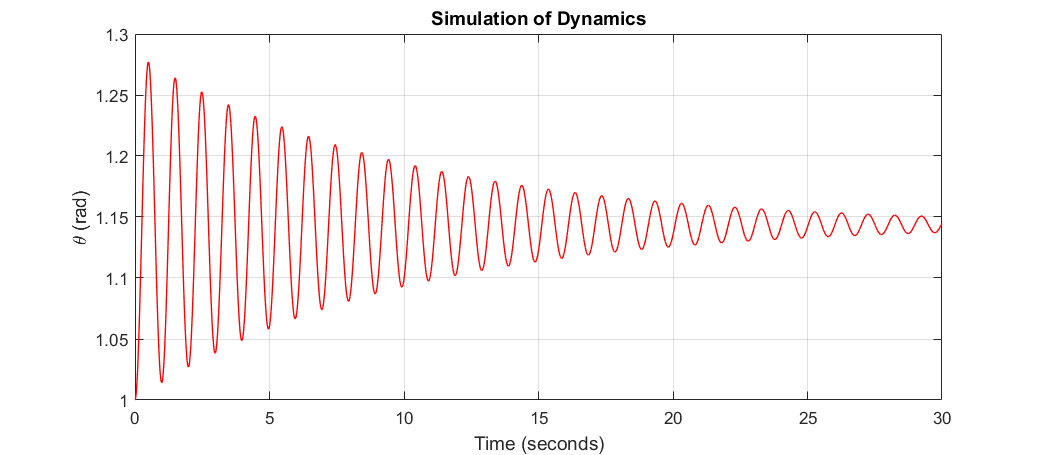
\includegraphics[width=1\textwidth]{pics/simulation.png}
		\end{figure}
	\end{figure}
\end{frame}

%\subsection{SimMechanics}
%\begin{frame}{Simulation}
%	\framesubtitle{SimMechanics}
%	Eventuelle Erfolge mit SimMechanics werden hier dargestellt werden.
%\end{frame}
\section{Task 1: $h(\omega)$}
\subsection{Approach}
\begin{frame}{Task 1: $h(\omega)$}
	\framesubtitle{Approach}
	\centering Steady-State $\rightarrow$ $\dot{\theta} = \ddot{\theta} = 0$\\
	\begin{equation*}
		\frac{m_2}{2}\sin(2\theta)\omega^2 - \frac{g}{L}(m_1+m_2) \sin(\theta) = 0
	\end{equation*}
	\begin{equation*}
	\theta_e = 0 \quad \theta_e = \arccos\left(\frac{1}{\omega^2}\frac{g}{L}\frac{(m_1+m_2)}{m_2}\right)
	\end{equation*}
	\centering which can be substituted into $\vv{r}_{m1}$:
\end{frame}

\subsection{Result}
\begin{frame}{Task 1: $h(\omega)$}
	\framesubtitle{Result}
		\begin{figure}[H]
			\begin{equation*}
			h_{m1} = \begin{cases} 2L\left(1-\frac{1}{\omega^2}\frac{g}{L}\frac{(m_1+m_2)}{m_2}\right) & \omega > \sqrt{\frac{g}{L} \frac{m_1+m_2}{m_2}} \\ 0 & \text{else} \end{cases}
			\end{equation*}

		\end{figure}
\end{frame}

\subsection{Dependency}
\begin{frame}{Task 1: $h(\omega)$}
	\framesubtitle{Dependency}
	\begin{figure}[H]
		\centering
		$m_1 = 1\,\left[\mathrm{kg}\right]$, $m_2 = 2\,\left[\mathrm{kg}\right]$, $L = 0.4\,\left[\mathrm{m}\right]$\\
		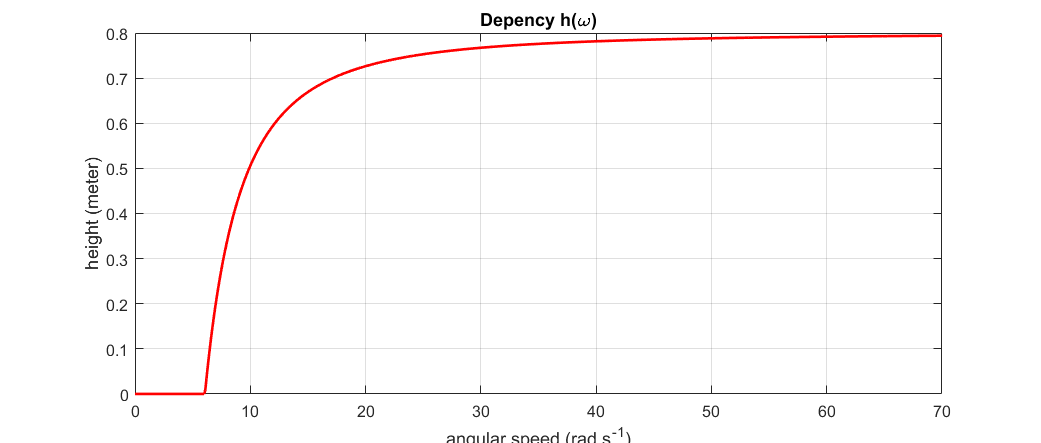
\includegraphics[width=1\textwidth]{pics/height.png}
	\end{figure}
\end{frame}



\section{Task 2: Frequency}
\subsection{Approach}
\begin{frame}{Task 2: Frequency}
	\framesubtitle{Ansatz}
	\begin{center}
		Small Oscillations around Steady-State
		\begin{equation*}
			\theta_e = 0 \quad \theta_e = \arccos\left(\frac{1}{\omega^2}\frac{g}{L}\frac{(m_1+m_2)}{m_2}\right)
		\end{equation*}
		Approximation with spring-mass-equation
		\begin{equation*}
			m\ddot{x} = -kx
		\end{equation*}
	\end{center}
\end{frame}


\subsection{Result}
\begin{frame}{Task 2: Frequency}
	\framesubtitle{Result}
	\begin{center}
		\begin{equation*}
			\Delta \ddot{\theta} = \frac{m_2\cos(2\theta_e)\omega^2 - \frac{g}{L}\cos(\theta_e)(m_1+m_2)}{m_1(1-\cos(2\theta_e))+m_2}\Delta \theta
		\end{equation*}
		\begin{align*}
			\omega_e =
			\sqrt{\frac{m_2\omega^2(g^2(m_1 + m_2)^2-L^2m_2^2\omega^4)}{2g^2m_1(m_1+m_2)^2-L^2m_2^2\omega^4(2m_1+m_2)}} 
		\end{align*}
		Edge Case: $m_1 = 0$
		\begin{equation*}
			\omega_e = \sqrt{\frac{L^2\omega^4 - g^2}{L^2\omega^2}}
		\end{equation*}
	\end{center}
\end{frame}

\subsection{Verification with simulation}
\begin{frame}{Task 2: Frequency}
	\framesubtitle{Verification with simulation}
	\begin{figure}[H]
		\centering
		$m_1 = 1\,\left[\mathrm{kg}\right]$, $m_2 = 2\,\left[\mathrm{kg}\right]$, $L = 0.4\,\left[\mathrm{m}\right]$, $\omega = 3\pi\,\left[\mathrm{\frac{rad}{s}}\right]$, $x_0 = \left(\begin{array}{c c}
		1 & 0
		\end{array}\right)^T \quad \text{Matlab: }1.01\,\left[\mathrm{Hz}\right]$\\ [0.5cm]
		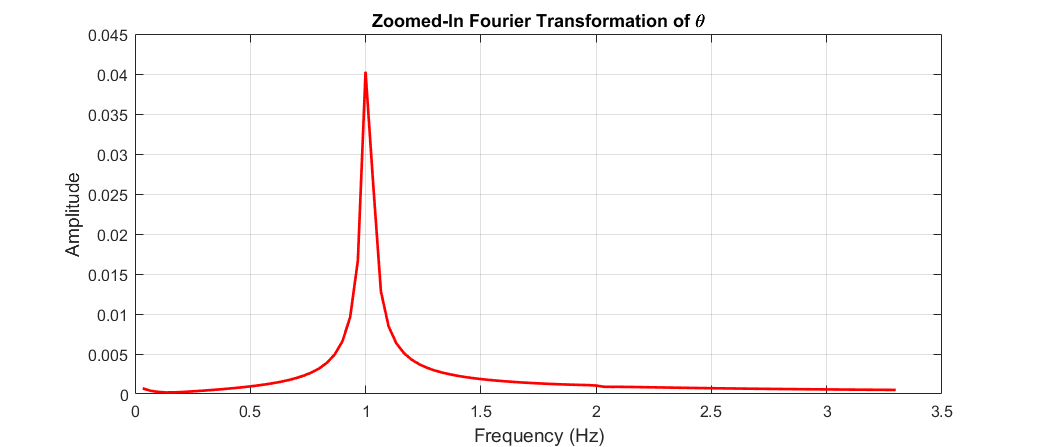
\includegraphics[width=1\textwidth]{pics/frequency.png}
	\end{figure}
\end{frame}
\end{document}